%%%%%%%%%%%%%%%%%%%%%%%%%%%%%%%%%%%%%%%%%%%%%%%%%%%
%
%  New template code for TAMU Theses and Dissertations starting Fall 2012.  
%  For more info about this template or the 
%  TAMU LaTeX User's Group, see http://www.howdy.me/.
%
%  Author: Wendy Lynn Turner 
%	 Version 1.0 
%  Last updated 8/5/2012
%
%%%%%%%%%%%%%%%%%%%%%%%%%%%%%%%%%%%%%%%%%%%%%%%%%%%

%%%%%%%%%%%%%%%%%%%%%%%%%%%%%%%%%%%%%%%%%%%%%%%%%%%%%%%%%%%%%%%%%%%%%%
%%                           SECTION I
%%%%%%%%%%%%%%%%%%%%%%%%%%%%%%%%%%%%%%%%%%%%%%%%%%%%%%%%%%%%%%%%%%%%%


\pagestyle{plain} % No headers, just page numbers
\pagenumbering{arabic} % Arabic numerals
\setcounter{page}{1}


\chapter{\uppercase {\textit{UBE3A} imprinting in neurons: a unique model for antisense lncRNA regulation}}

The genomic instability of chromosome 15q11-q13 results in multiple disorders, two of which seems to be linked to ubiquitin ligase E3A protein (UBE3A) expression, also known as E6AP, \cite{Christian1999,Kishino1997,Matsuura1997,Nurmi2001}. The non-Mendelian inheritance of these disorders are a result of genomic imprinting, an epigenetic phenomenon that results in the differential expression of diploid alleles in a parent-of-origin specific manner \cite{Russo1996}. With respect to \textit{UBE3A}, it is clear that expression and dosage levels are important for human brain development and functionality. As such, the unique imprinting of \textit{UBE3A} in only neurons is perplexing. Although it is possible that the imprint could be an innocent bystander, the fact that it has been evolutionarily constrained for over 100 million years suggests otherwise \cite{Rapkins2006}. The focus of this review is to examine the functional significance of the imprinting mechanism of \textit{UBE3A} and the roles antisense long non-coding RNA (lncRNA) play in regulation of the sense transcripts.

\section{Diseases of Chromosome 15q11-q13}

The long arm of human chromosome 15 is characterized by relatively frequent chromosome rearrangements, which are due to low-copy repeat elements at two proximal and one distal region of the 15q11-q13 region \cite{Amos-Landgraf1999,Ji2000,Ji1999,Pujana2001}. \textbf{Figure \ref{Figure 1-1: }} depicts the breakpoint locations around the \textit{HERC2} (HECT, homologous to the E6AP carboxyl terminus, and RDL, regulator of chromosome condensation 1 (RCC1) like domain, domain containing E3 ubiquitin protein ligase 2) duplicons and the percentage of usages within the large-scale deletions. This instability results in multiple structural abnormalities, including deletions, duplications, and translocations \cite{Buiting1998,Christian1999,Jiang2008,Pujana2002,Webb1994} resulting in three distinct neurodevelopmental disorders: Prader-Willi syndrome (PWS), Chromosome 15q11-q13 Duplication syndrome (Dup15q) and Angelman syndrome (AS).

%%%%%%%%%%%%%%%%%%%%%%%%%%%%%%%%%%%%%%%%%%%%%%%%%%%%%%
\begin{sidewaysfigure}
\centering
\resizebox{\linewidth}{!}{
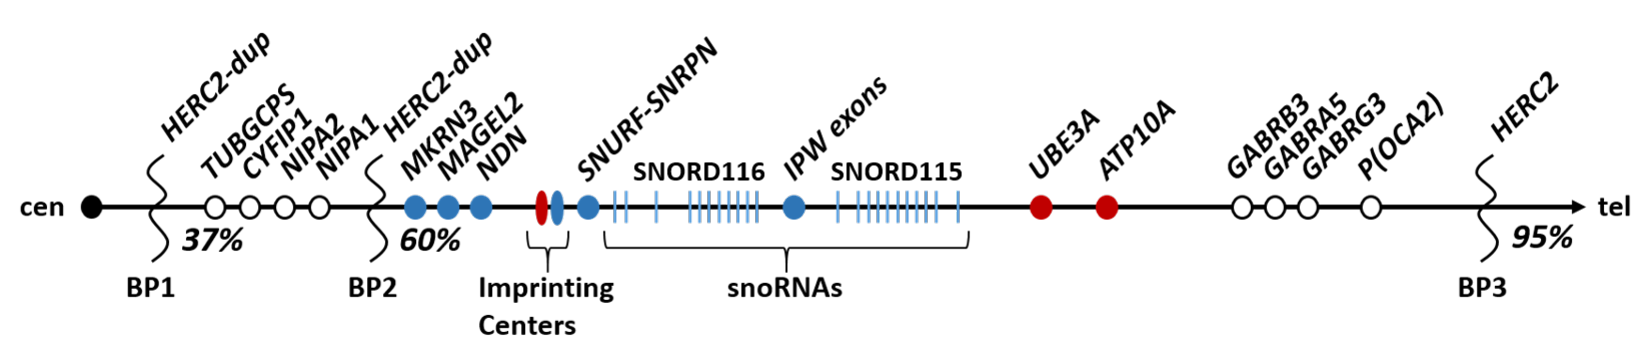
\includegraphics{figures/15q11-q13_region2.pdf}
}
\caption{The frequent rearrangements of human chromosome 15q11-q13 region is due to recombination hotspots of the \textit{HERC2} duplicons at the three breakpoints (BP). Paternally expressed genes in blue, maternally expressed genes in red, and biallelically expressed genes in white.}
\label{Figure 1-1: }
\end{sidewaysfigure}
%%%%%%%%%%%%%%%%%%%%%%%%%%%%%%%%%%%%%%%%%%%%%%%%%%%%%%
\subsection{Prader-Willi Syndrome}

Prader-Willi syndrome (OMIM \#176270) is characterized by neonatal hypotonia and failure to thrive, hyperphagia in early childhood leading to obesity, hypogonadism, short stature, behavior problems, and mild to moderate intellectual disability \cite{Cassidy2012,Goldstone2004}. The genetic or epigenetic mutations causing PWS are associated with the specific loss of paternal expression of the box C/D small nucleolar RNAs (snoRNAs) generated from \textit{SNORD116} cluster (previously referred as \textit{HBII-85}) in the brain \cite{Bortolin-Cavaille2012,Ding2008,Duker2010}. The spectrum of mutations causing PWS include:
(i) paternal interstitial deletions of 15q11-q13 region,
(ii) maternal uniparental disomy of chromosome 15,
(iii) genomic imprinting defects of the region, or
(iv) loss-of-function mutations in \textit{SNORD116} gene cluster \cite{Cassidy2012}.

\subsection{Chromosome 15q11-q13 Duplication Syndrome}

Chromosome 15q11-q13 duplication syndrome (OMIM \#608636) is characterized by developmental delay, intellectual disability, early central hypotonia, seizures, and social impairment \cite{Battaglia2008}. Additionally, duplication of 15q11-q13 is one of the most common genetic mutations observed in individuals diagnosed with autism spectrum disorder \cite{Battaglia2008,Bolton2001,Cook1997,Nurmi2001,Schroer1998}. Chromosome 15q duplication syndrome is primarily caused by maternal duplications of chromosome 15q11-q13 \cite{Battaglia2008,Browne1997}. Currently, Dup15q is known to occur via one of two ways:
interstitial duplication of 15q,
or extra isodicentric chromosome of 15q \cite{Battaglia2008,Klei2012}. As the neurodevelopmental disorder is caused by maternal inheritance of duplications, it is linked to the overexpression of ubiquitin ligase E3A protein (UBE3A) \cite{Nurmi2001}.

\subsection{Angelman Syndrome}

Angelman syndrome (OMIM \#105830) is a debilitating neurodevelopmental disorder characterized by severe intellectual disability, absent speech, ataxia, seizures, frequent smiling and inappropriate laughter \cite{Williams2006}. Although clinically distinct, AS shares a common pathogenesis with Dup15q, namely dysregulation of UBE3A protein. In contrast to Dup15q, the genetic or epigenetic mutations causing AS are associated with the specific loss of maternal expression of UBE3A protein in the brain \cite{Kishino1997,Matsuura1997,Williams2006}. The spectrum of mutations causing AS include:
(i) maternal interstitial deletions of 15q11-q13 region,
(ii) paternal uniparental disomy of chromosome 15,
(iii) genomic imprinting defects of 15q11-q13, or
(iv) loss-of-function mutations in the \textit{UBE3A} gene \cite{Williams2006}.

\section{Ubiquitin Ligase E3A Protein Gene}

The \textit{UBE3A} gene is located within the 15q11-q13 imprinted domain and encodes an E3 ubiquitin-protein ligase that is a central component of the ubiquitin proteasome system involving the successive action of E1 (ubiquitin-activating), E2 (ubiquitin-conjugating), and E3 ubiquitin-protein ligases activities \cite{Huibregtse1995,Scheffner1995}. The UBE3A protein is a unique ligase as it can catalyze the formation of isopeptides via its HECT domain without the help of E2 proteins. In addition, UBE3A has been shown to function as a typical ubiquitin ligase and a transcriptional coactivator of steroid hormone receptors \cite{Kumar1999,Sun2012}. Thus far, numerous cellular proteins have been shown to interact directly or indirectly with UBE3A suggesting that is has diverse cellular functions (\textbf{APPENDIX A, Tables \ref{table:a-1}, \ref{table:a-2}} and {\textbf{\ref{table:a-3}}).

\subsection{\emph{UBE3A} in Neurons}

The non-Mendelian inheritance pattern of AS is due to genomic imprinting of \textit{UBE3A} \cite{Kishino1997,Matsuura1997}; however, \textit{UBE3A}, unlike most imprinted genes, is expressed from both parental alleles in almost all cell types except for neurons \cite{Landers2004,Rougeulle1998,Runte2004,Yamasaki2003}. Expression of the paternal \textit{UBE3A} allele in neurons is inhibited by the antisense expression of a long polycistronic transcriptional unit that is comprised of \textit{SNURF-SNRPN}, clusters of C/D box snoRNAs (\textit{SNORD116} and \textit{SNORD115}), and \textit{UBE3A} antisense transcript (\textit{UBE3A-AS}) \cite{Landers2004,Meng2012,Meng2013,Runte2001,Runte2004}. \textbf{Figure \ref{Figure 1-2: }} shows the polycistronic transcriptional unit transcribed from the paternal allele (blue) with the overlapping antisense transcript silencing \textit{UBE3A} (black).

%%%%%%%%%%%%%%%%%%%%%%%%%%%%%%%%%%%%%%%%%%%%%%%%%%%%%%
\begin{sidewaysfigure}[p]
\centering
\resizebox{\linewidth}{!}{
  
  \begin{tikzpicture}[highline/.style={above=3pt,text height=1.5ex,text depth=0.25ex,font={\large \itshape}},
      pgene/.style={line width=4pt, blue},
      topline/.style={above=2pt,text height=1.5ex,text depth=0.25ex,font={\Large \bfseries}},
      bottomline/.style={below=7pt,text height=1.5ex,text depth=0.25ex,font={\Large \bfseries}}]
      
    %draw horizontal line
    \draw[line width=4pt] (-0.078,0) -- (30,0);

    %draw PTU arrow and labels
    \draw[line width=2pt] (0.75, 50pt) -- (0.75, 0pt);
    \draw[->,shorten >= 1pt,>=stealth', line width=2pt] (0.75,49pt) -- (1.6,49pt);
    \draw[->,shorten >= 1pt,>=stealth', line width=2pt] (1.65, 49pt) -- (30, 49pt);
    \draw[-|, dashed, line width=2pt] (28.0, 46pt) to[out=135,in=90] (28.5, 24pt);
    
    \draw (1.5, 50pt)   node[highline] {PTU};
    \draw (13.25, 50pt) node[highline] {SNORD116-HG};
    \draw (18.35, 50pt) node[highline] {IPW};
    \draw (22.8, 50pt)  node[highline] {SNORD115-HG};
    \draw (27.7, 50pt)  node[highline] {UBE3A-AS};
    
    %draw U-exons
    \draw[pgene] (1.3, 20pt) -- (1.3, -20pt);
    \draw[pgene] (1.7, 20pt) -- (1.7, -20pt);
    \foreach \x in {2, 2.2, ..., 3}{
      \draw[pgene] (\x, 20pt) -- (\x,-20pt);
    }
    \draw (2.15, -20pt) node[bottomline] {U-exons};

    %draw ICR
    \draw[line width=1.5pt] (3.7, 25pt) -- (3.7, 0pt);
    \draw[line width=1.5pt] (3.8, 25pt) -- (3.8, 0pt);
    \draw[line width=1.5pt, fill=white] (3.75, 29pt) ellipse (8pt and 6pt);
    \draw (3.65, 0pt) node[below = 2pt, xshift=2pt, font={\Large}] {ICR};

    %draw SNURF-SNRPN
    \draw[pgene] (4.5, 20pt) -- (4.5, -20pt);
    \draw[pgene] (4.8, 20pt) -- (4.8, -20pt);
    \draw[rounded corners=10pt,fill=blue,blue] (5.1,20pt) rectangle (9.2,-20pt);
    \draw[line width=2pt] (5.06, 35pt) -- (5.06, 0pt);
    \draw[->,shorten >= 1pt,>=stealth', line width=2pt] (5.06,34pt) -- (6.0,34pt);
    \draw (7.0, -20pt) node[bottomline] {SNURF-SNRPN};

    %draw SNORD116 Cluster
    \foreach \x in {10.5, 10.8, ..., 12.9}{
      \draw[pgene, line cap=round] (\x, 19pt) -- (\x,-19pt);
    }
    \foreach \x in {13.6, 13.9, ..., 16.0}{
      \draw[pgene, line cap=round] (\x, 19pt) -- (\x,-19pt);
    }
    \draw (13.25, 20pt) node[topline] {SNORD116 Cluster};

    %draw IPW
    \draw[rounded corners=10pt,fill=blue,blue] (17.5, 20pt) rectangle (19.3, -20pt);
    \draw (18.4, -20pt)  node[bottomline] {IPW};

    %draw SNORD115 Cluster
    \foreach \x in {20.8, 21.1, ..., 25.0}{
      \draw[pgene, line cap=round] (\x, 19pt) -- (\x,-19pt);
    }
    \draw (22.8, 20pt) node[topline] {SNORD115 Cluster};

    %draw UBE3A and UBE3A-AS
    \draw[rounded corners=10pt,fill=black] (26.5, 20pt) rectangle (29.0, -20pt);
    \draw (27.8, -20pt) node[bottomline] {UBE3A};
    
  \end{tikzpicture}
}

\caption{Paternal expression of long alternatively spliced transcript in neurons comprising \textit{SNURF/SNRPN}, C/D box snoRNAs (\textit{SNORD116} and \textit{SNORD115}), \textit{IPW}, and \textit{UBE3A-AS} is controlled by unmethylated Prader-Willi syndrome imprinting center region (ICR). There some unknown mechanism \textit{UBE3A-AS} inhibits expression of paternal \textit{UBE3A}. Paternally expressed genes in blue and paternally silenced \textit{UBE3A} in black.}
\label{Figure 1-2: }
\end{sidewaysfigure}
%%%%%%%%%%%%%%%%%%%%%%%%%%%%%%%%%%%%%%%%%%%%%%%%%%%%%%

\section{Genomic Imprinting}

Mammals are diploid organisms that inherit a chromosome set from each parent. As a result, the majority of genes are expressed from both parents; however, a subset of genes show parent-specific gene expression due to epigenetic modifications. \textbf{Figure \ref{Figure 1-3: }} depicts normal biallelic expression compared to the monoallelic expression of imprinted genes. There are over a 100 of these imprinted genes in mouse and humans \cite{Radford2011,Santoro2011}; the majority of which are found within gene clusters that house at least one non-coding RNA and several protein coding genes.

%%%%%%%%%%%%%%%%%%%%%%%%%%%%%%%%%%%%%%%%%%%%%%%%%%%%%%
\begin{figure}[!ht]
\centering
  \resizebox{\linewidth}{!}{
    \begin{tikzpicture}[every node/.style={minimum size=2em, inner sep=0}]
      \node(scope1){
              
        \begin{tikzpicture}[rnamat/.style={line width=2pt, red!80!black},
            rnapat/.style={line width=2pt, blue!80!black}]
                
          %draw maternal allele
          \draw[line width=4pt] (-0.078,0) -- (10,0);
          \draw[rounded corners=10pt,fill=red,red] (1.4,20pt) rectangle (8.6,-20pt);
          \draw[line width=4pt] (1.33, 40pt) -- (1.33, 0pt);
          \draw[->,shorten >= 0.5pt,>=stealth', line width=4pt] (1.32,38pt) -- (2.7,38pt);
          \draw (5, 0pt) node[text centered,font={\Huge \bfseries}] {Gene X};
                
          %RNA expression maternal allele
          \draw[rnamat] (9.8,42pt)  -- (11,42pt);
          \draw[rnamat] (10.8,36pt) -- (12,36pt);
          \draw[rnamat] (9.6,32pt)  -- (10.8, 32pt);
          \draw[rnamat] (10.9,29pt) -- (12.1,29pt);
          \draw[rnamat] (9.8,25pt)  -- (11,25pt);
          \draw[rnamat] (10.6,20pt) -- (11.8,20pt);
                
          %draw paternal allele
          \draw[line width=4pt] (-0.078,-80pt) -- (10,-80pt);
          \draw[rounded corners=10pt,fill=blue!60!white,blue!60!white] (1.4,-60pt) rectangle (8.6,-100pt);
          \draw[line width=4pt] (1.33, -40pt) -- (1.33, -80pt);
          \draw[->,shorten >= 1pt,>=stealth', line width=4pt] (1.32,-42pt) -- (2.7,-42pt);
          \draw (5, -80pt) node[text centered,font={\Huge \bfseries}] {Gene X};
                
          %RNA expression maternal allele
          \draw[rnapat] (9.8,-38pt)  -- (11,-38pt);
          \draw[rnapat] (10.8,-44pt) -- (12,-44pt);
          \draw[rnapat] (9.6,-48pt)  -- (10.8,-48pt);
          \draw[rnapat] (10.9,-51pt) -- (12.1,-51pt);
          \draw[rnapat] (9.8,-55pt)  -- (11,-55pt);
          \draw[rnapat] (10.6,-60pt) -- (11.8,-60pt);
                
          \draw (10.85,60pt) node[text centered,font={\Large \itshape}] {RNA expression};
          \draw (5.5, 95pt)    node[text centered,font={\Huge \bfseries}] {Biallelic Expression};

    \end{tikzpicture}
  };
  \node[right= 2mm of scope1] (scope2){
    
    \begin{tikzpicture}[rnamat/.style={line width=2pt, red!80!black},
        rnapat/.style={line width=2pt, blue!80!black}]
          %draw maternal allele
          \draw[line width=4pt] (-0.078,0) -- (10,0);
          \draw[rounded corners=10pt,fill=red,red] (1.4,20pt) rectangle (8.6,-20pt);
          \draw[line width=4pt] (1.33, 40pt) -- (1.33, 0pt);
          \draw[line width=4pt] (1.32,38pt) -- (2.7,38pt);
          \draw (2.35,37.5pt) node[text centered,font={\LARGE \bfseries \sffamily}] {X};
          \draw (3.2, 0pt) node[text centered,font={\Huge \bfseries}] {Gene X};
                
          %draw paternal allele
          \draw[line width=4pt] (-0.078,-80pt) -- (10,-80pt);
          \draw[rounded corners=10pt,fill=blue!60!white,blue!60!white] (1.4,-60pt) rectangle (8.6,-100pt);
          \draw[line width=4pt] (1.33, -40pt) -- (1.33, -80pt);
          \draw[->,shorten >= 0.5pt,>=stealth', line width=4pt] (1.32,-42pt) -- (2.7,-42pt);
          \draw (3.2, -80pt) node[text centered,font={\Huge \bfseries}] {Gene X};
                
          %RNA expression maternal allele
          \draw[rnapat] (9.8,-38pt)  -- (11,-38pt);
          \draw[rnapat] (10.8,-44pt) -- (12,-44pt);
          \draw[rnapat] (9.6,-48pt)  -- (10.8,-48pt);
          \draw[rnapat] (10.9,-51pt) -- (12.1,-51pt);
          \draw[rnapat] (9.8,-55pt)  -- (11,-55pt);
          \draw[rnapat] (10.6,-60pt) -- (11.8,-60pt);

          %draw ICR
          \draw[line width=2pt] (0.5, 25pt) -- (0.5, 0pt);
          \draw[line width=2pt] (0.7, 25pt) -- (0.7, 0pt);
          \draw[line width=1pt, fill=black] (0.6, 29pt) ellipse (9pt and 7pt);

          \draw[line width=2pt] (0.5, -55pt) -- (0.5, -80pt);
          \draw[line width=2pt] (0.7, -55pt) -- (0.7, -80pt);
          \draw[line width=1pt, fill=white] (0.6, -51pt) ellipse (9pt and 7pt);
          
          \draw (8.85,60pt) node[text centered,font={\Large \itshape}] {RNA expression};
          \draw (0.5, 95pt)    node[text centered,font={\Huge \bfseries}] {Monoallelic Expression};
    \end{tikzpicture}
  };
  
\end{tikzpicture}
}
\caption{The majority of genes show biallelic expression with maternal (red) and paternal (blue) alleles expressed in all tissues. In a subset of genes via some epigenetic mechanism such as DNA methylation, gene expression is limited to monoallelic expression. \drawICR[fill=black] is methylated ICR, and \drawICR[fill=white] is unmethylated ICR.}
\label{Figure 1-3: }
\end{figure}
%%%%%%%%%%%%%%%%%%%%%%%%%%%%%%%%%%%%%%%%%%%%%%%%%%%%%%

\subsection{Imprinting Control Regions}

Epigenetics is defined as heritable modifications of the genome that are not genetic changes (e.g. DNA and chromatin modifications) \cite{Bird2007}. As imprinting is an epigenetic phenomenon, the imprinted genes must be able to acquire modifications, maintain imprinting status, and be re-established in the germline. For imprinted gene clusters, large-range \textit{cis}-acting imprinting control regions (ICRs) are responsible for acquiring parental modification and maintaining imprinting status \cite{Edwards2007,Edwards2007a,Spahn2003}. All ICRs have differential DNA methylation regions (DMR), which carry parental information \cite{Ciccone2009}.

The ICR for PWS and AS has a bipartite structure comprising the Prader-Willi and Angelman syndrome imprinting centers (PWS-IC and AS-IC); thus, giving this ICR bidirectional control of the cluster of imprinted genes in the 15q11-q13 region \cite{Nicholls1996}. The PWS-IC is a positive regulatory element responsible for the establishment and maintenance of paternal gene expression \cite{Nicholls2001}, while AS-IC negatively regulate PWS-IC on the maternal chromosome \cite{Brannan1999}.

Differential methylation is associated with a CpG island surrounding the promoter and exon 1 of \textit{SNRPN} \cite{Blaydes1999}. In somatic cells of human and mouse, PWS-IC is heavily CpG methylated on the maternal chromosome, and is almost completely unmethylated on the paternal chromosome \cite{Glenn1996,Shemer1997}. The AS-IC on the maternal allele confers DNA methylation and suppression of PWS-IC, but is methylated and inactive on the paternal allele. This results in PWS-IC regulation of the majority of the genes as paternal expression expect for \textit{UBE3A} and \textit{ATP10A}, which are maternally expressed \cite{Brannan1999, Kantor2006}.

\section{Function of Imprinting}

No matter the theory, the overall result of imprinting is the differential silencing of alleles. This imprinting does not happen by chance as it is often evolutionary conserved between mouse and humans. For example, the imprinted cluster within 15q11-q13 arose 105-180 million years ago \cite{Rapkins2006}; and despite the disease phenotypes and genomic instability associated with the region, it remains conserved. For some reason, it is advantageous to imprint this gene cluster and many others. One method to explore what makes the imprinting of gene clusters advantageous, is to investigate the function of the imprinted genes. Are the genes dosage sensitive? Does the imprint increase regulatory function? For the 15q11-q13 imprinting cluster, these answers are not readily apparent.

\subsection{Dosage Regulation}

Why \textit{Ube3a} became imprinted in neurons is unclear. The current theory is that \textit{Ube3a-AS} evolved to reduce \textit{Ube3a} expression in neurons to regulate dosage because termination of \textit{Ube3a-AS} leads to increased levels of Ube3a expression in the brain \cite{Huang2012,King2013,Meng2013}. When our laboratory rigorously tested this theory, we determined that the function of the imprinting mechanism was not to reduce the expression of Ube3a in the brain, as there was no correlation between the imprint and expression levels of \textit{Ube3a/UBE3A} in mouse and human \cite{Hillman2017}. Additionally, while the paternal \emph{Ube3a} allele was silenced the maternal allele was upregulated during development so that overall Ube3a expression remained unchanged \cite{Hillman2017}. Altogether, the findings suggest that imprinting of Ube3a in neurons may have evolved for reasons other than to reduce Ube3a expression in neurons.

\subsection{Regulatory Function}

The evolution of \textit{SNRPN} is a good example of a duplication event leading to tissue-specific imprinting with alternative function from its ancestor gene, \textit{SNRPB/B’}. Studies have shown that \textit{Snrpn} originated from \textit{Snrpb}, a small nuclear ribonucleoprotein (snRNP) gene encoding for SmB in mice, locus via a duplication event about 180-210 million years ago \cite{Gray1999,Rapkins2006}. While SmB is replaced by SmN in the brain, \textit{SNRPB/B’} is upregulate in the absence of \textit{SNRPN} suggesting that the two genes are tightly regulated \cite{Gray1999,Nahkuri2008}. Despite their similarities, \textit{SNRPB/B’} and \textit{SNRPN} have distinct snRNP association along with tissue-specific expression, suggesting that \textit{SNRPN} has evolved an alternative function compared to its ancestral gene \cite{Huntriss1993}.

Given the current findings, \textit{Ube3a} does not appear to be imprinted as a mechanism to regulate dosage in neurons. With that in mind it is possible that \textit{Ube3a} is imprinted in neurons because of additional regulatory functions. While \textit{Ube3a} is highly expressed in the brain, the imprint has no effect on overall expression \cite{Hillman2017}. Therefore, it is unlikely that the imprint of \textit{Ube3a} is directly linked to Ube3a protein expression; however, its long non-coding antisense RNA transcript, \textit{Ube3a-AS}, arises only in neurons as part of the imprinting mechanism of \textit{Ube3a}. Further study of this transcript may reveal the functional reason for imprinting Ube3a in neurons.

\section{Long Non-Coding RNA}

Over the last few decades, the scientific community has increasingly become fascinated with non-coding RNAs (ncRNAs), especially long non-coding RNAs (lncRNA), and with good reason. With the advancement of genomic sequencing technologies, numerous annotations and deep sequencing from multiple species have demonstrated that ncRNAs are more abundant than protein-coding genes \cite{Clark2011,Kapranov2007a}. To put this in perspective, of the 75-90\% of the human genome that is transcribed, only 3\% is protein-coding \cite{Carninci2005,Consortium2012,Djebali2012,Guttman2009,Kapranov2007}. More importantly, this is not transcriptional noise as these ncRNAs perform a myriad of functions by interacting with DNA, RNA, and proteins similar to protein-coding genes \cite{Mattick2005,Mercer2009}. The importance of ncRNAs extends to genomic imprinting as well since all ICRs have at least one lncRNA expressed from the unmethylated parental chromosome \cite{Lee2013,Mohammad2009,Sleutels2002}. Even with the clear importance of ncRNA, the function of the majority of ncRNAs, especially lncRNAs, is unknown.

Recently, the importance of ncRNAs in tissue- and developmental stage-specific gene expression has been extensively explored. Moreover, increasing evidence implements them in brain development, synaptic plasticity, and neurological disease, with the highest proportion of tissue-specific lncRNA expression in the brain \cite{Derrien2012,Washietl2014}. Long non-coding RNAs are less understood. With no common sequence or structure, classification is difficult. In general, lncRNA preform many similar roles as ncRNAs, like microRNAs and small interfering RNAs, and are separate from ncRNAs via size ($>$ 200 bp). A simplistic classification of lncRNAs uses loci-of-origin resulting in several different categories, three of which, enhancer RNAs, overlapping RNAs, and intergenic RNAs, are depicted in \textbf{Figure \ref{Figure 1-4: }}. These three types of lncRNA are all present within ICRs \cite{Bartolomei1991,Darrow2013,Katayama2005,Wevrick1997,Wevrick1994}, with some of the most well-studied lncRNAs in ICRs being antisense lncRNA.

%%%%%%%%%%%%%%%%%%%%%%%%%%%%%%%%%%%%%%%%%%%%%%%%%%%%%%
\begin{figure}%[h]
\centering
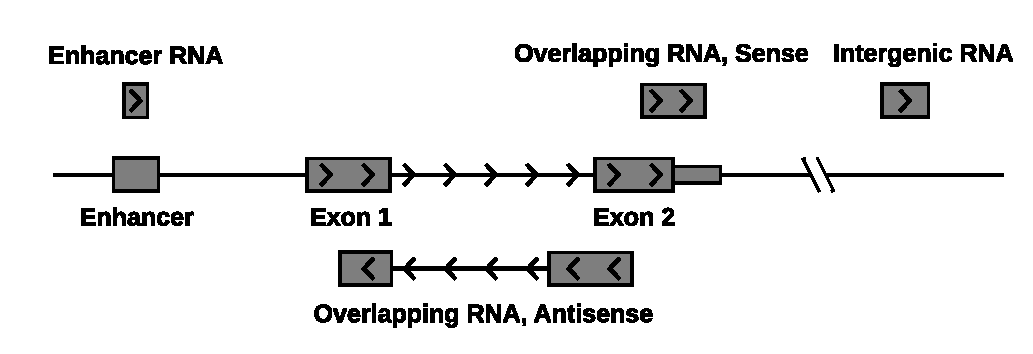
\includegraphics[scale=0.85]{figures/lncRNAs2.pdf}
\caption{Schematic of lncRNAs based on loci-of-origin depicting an enhancer RNA, sense and antisense overlapping RNAs, and an intergenic RNA.}
\label{Figure 1-4: }
\end{figure}
%%%%%%%%%%%%%%%%%%%%%%%%%%%%%%%%%%%%%%%%%%%%%%%%%%%%%%

\section{Antisense lncRNA}

Natural antisense transcripts are endogenous transcripts with complete or partial overlap of genes or ncRNA that can work in \textit{cis} or \textit{trans}. Sense/antisense pairings can be non-coding or protein-coding; however, the majority of pairs are non-coding antisense regulating protein-coding sense \cite{Katayama2005}. Of the protein-coding sense transcripts, a majority (~70\%) have antisense pairings, many of which are lncRNAs \cite{Beiter2009,Carlile2009}. Furthermore, sense/antisense origination is more likely to be conserved than gene pairs on the same strand, suggesting a conserved functional significance \cite{Dahary2005}. This functional conservation is observed in their diverse structure, expression pattern, and methods of regulation \cite{Pelechano2013}, such as direct regulation of transcription (i.e. transcriptional interference), epigenetic regulation (i.e. genomic imprinting), nucleus interactions (i.e. alternative splicing and termination), and cytoplasmic interaction (i.e. mRNA stability and masking microRNA binding sites).

%%%%%%%%%%%%%%%%%%%%%%%%%%%%%%%%%%%%%%%%%%%%%%%%%%%%%%
\begin{figure}[!ht]
\centering
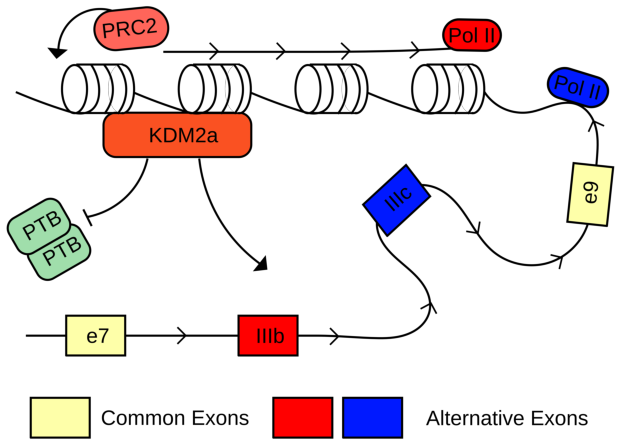
\includegraphics[scale=1]{figures/FGFR2-AS2.pdf}
\caption{\emph{FGFR2-AS} plays a central role in tissue-specific alternative splicing of \emph{FGFR2} via chromatin remodeling. The \emph{FGFR2} antisense transcript recruits PRC2 and KDM2a, which interfere with PTB repression of exon IIIb, resulting in exclusion of exon IIIc. PolII, polymerase II, antisense in red and sense strand in blue.}
\label{Figure 1-5: }
\end{figure}
%%%%%%%%%%%%%%%%%%%%%%%%%%%%%%%%%%%%%%%%%%%%%%%%%%%%%%


\subsection{\textit{FGFR2-AS}}

Antisense transcript of \textit{FGFR2} (\textit{FGFR2-AS}), human fibroblast growth factor receptor 2, is a recently discovered antisense lncRNA of approximately 875 bp that starts 282 bp upstream exon IIIc of \textit{FGFR2} gene \cite{Gonzalez2015}. \textit{FGFR2} exhibits chromatin to tissue-specific alternative splicing via chromatin-splicing adaptor system (MRG15), which recognizes H3K36me2,3 to inhibit inclusion of alternative splicing exon IIIb, and protein-protein interaction recruiting PTB (polypyrimidine tract binding protein) to exon IIIb (negative splicing regulatory element) \cite{Luco2010,Zhang2006}. Only recently has \textit{FGFR2} been shown to have an antisense transcript that does not appear to be spliced or polyadenylated \cite{Gonzalez2015}. Gonzalez and company determined that this evolutionary conserved antisense transcript is located predominantly in the nucleus, where it plays a role in alternative splicing of \textit{FGFR2} sense gene. Additionally, the group demonstrated that \textit{FGFR2-AS} inhibits repression of exon IIIb by interfering with PTB recruitment as shown in \textbf{Figure \ref{Figure 1-5: }}. In doing so, \textit{FGFR2-AS} recruits PRC2 (polycomb repressive complex 2) and KDM2a, a histone demethylase, to modulate splicing. Furthermore, demonstrating that this process is dependent on chromatin remodeling suggesting a central role in tissue-specific alternative splicing for \textit{FGFR2-AS}.

\subsection{\textit{Airn}}

\textit{Airn} (antisense to \textit{Igf2r} RNA non-coding), a 108 kbp paternally expressed lncRNA, is responsible for the silencing of the three maternally expressed protein-coding genes, \textit{Igf2r}, \textit{Slc22a2}, and \textit{Slc22a3} within the \textit{Igf2r} gene cluster. Expression of \textit{Airn} is responsible for the silencing of overlapping \textit{Igf2r} and non-overlapping \textit{Slc22a2} and \textit{Slc22a3} in \textit{cis} \cite{Sleutels2002} as shown in \textbf{Figure \ref{Figure 1-6: }}. For \textit{Slc22a2} and \textit{Slc22a3}, \textit{Airn} recruits chromatin modifiers in a sequence-specific manner to their promoters \cite{Nagano2008}. Interestingly, \textit{Airn} must be continuously transcribed to silence overlapping \textit{Igf2r} until the \textit{Igf2r} promoter is irreversibly silenced by CpG methylation, which is sufficient to maintain the imprint \cite{Latos2012,Santoro2013}. How chromatin and DNA modifiers are recruited to the \textit{Igf2r} promoter, and what role the antisense transcript plays, if any, in its recruitment remains unclear.

%%%%%%%%%%%%%%%%%%%%%%%%%%%%%%%%%%%%%%%%%%%%%%%%%%%%%%
\begin{figure}[!ht]
\centering
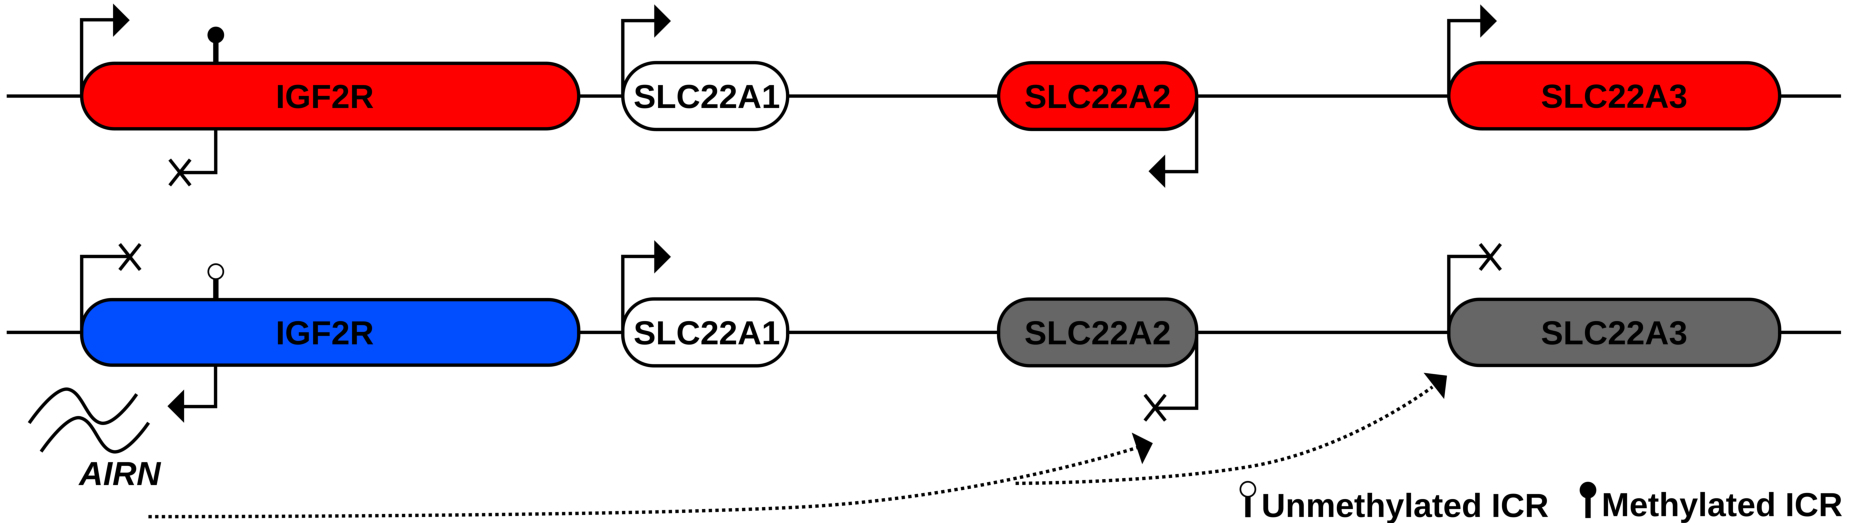
\includegraphics[scale=0.45]{figures/AIRN2.pdf}
\caption{Transcription of \emph{AIRN} regulates transcriptional gene silencing of the \emph{IGF2R} gene cluster. Continuous \emph{AIRN} transcription silences \emph{IGF2R} by transcriptional overlap of \emph{IGF2R} promoter. By some unknown mechanism, the \emph{IGF2R} promoter is irreversibly methylated. Silencing of \emph{SLC22A2} and \emph{SLC22A3} occurs through \emph{AIRN}-mediated recruitment of chromatin modifiers to their promoters. Maternal allele (red), paternal allele (blue), silenced genes (gray), and non-imprinting genes (white). Arrows denote direction of transcription.}
\label{Figure 1-6: }
\end{figure}
%%%%%%%%%%%%%%%%%%%%%%%%%%%%%%%%%%%%%%%%%%%%%%%%%%%%%%

\subsection{\textit{Nespas}}

\textit{Nespas}, a 27 kbp lncRNA, is a paternally expressed antisense lncRNA belonging to the \textit{Gnas} imprinting cluster containing four sense transcripts: \textit{Nesp}, \textit{Gnasxl}, \textit{Exon1A}, and \textit{Gnas} \cite{Kelsey1999,Peters1999,Williamson2004,Williamson2002}. \textit{Nesp} is maternally expressed in all tissues \cite{Egrie2001,Peters2006}, and imprinted expression is controlled by paternally methylated \textit{Nesp} DMR and maternally methylated \textit{Nespas-Gnasxl} DMRs, which contains promoters for \textit{Nespas} and \textit{Gnasxl} \cite{Coombes2003,Williamson2006}. The paternal restricted expression of \textit{Nespas} is due to methylation of the maternal \textit{Nespas} promoter \cite{Bliek2009,Holmes2003}. \textbf{Figure \ref{Figure 1-7: }} depicts the silencing of paternal \textit{Nesp} via \textit{Nespas} transcriptional overlap of the \textit{Nesp} promoter resulting in the recruitment of H3K4me3, which methylates the \textit{Nesp} promoter \cite{Ball2013,Tibbit2015,Williamson2011,Williamson2002,Wroe2000}.

%%%%%%%%%%%%%%%%%%%%%%%%%%%%%%%%%%%%%%%%%%%%%%%%%%%%%%
\begin{figure}[!ht]
\centering
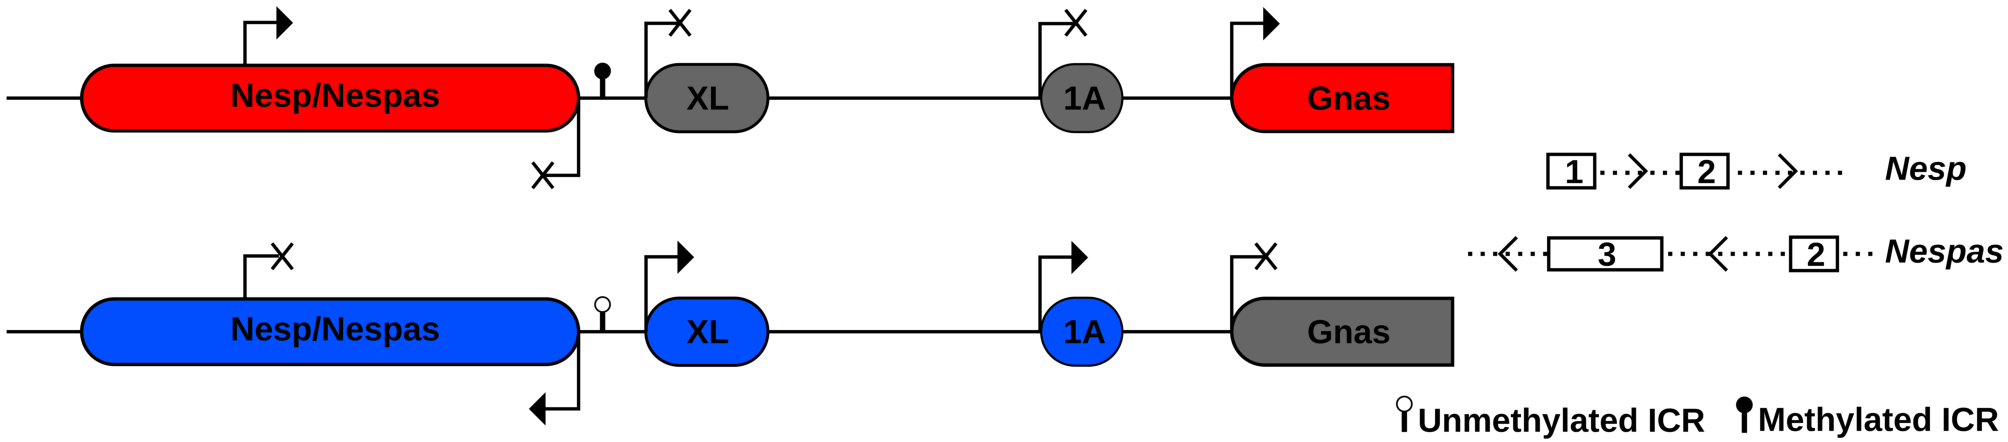
\includegraphics[scale=0.44]{figures/Nespas2.pdf}
\caption{\emph{Nespas} overlapping transcription occludes the \emph{Nesp} promoter, promoting CpG methylation silencing paternal expression of \emph{Nesp}. Maternal allele (red), paternal allele (blue), silenced genes (gray). Arrows denote direction of transcription. Zoom view of overlapping exons of \emph{Nesp} and \emph{Nespas}.}
\label{Figure 1-7: }
\end{figure}
%%%%%%%%%%%%%%%%%%%%%%%%%%%%%%%%%%%%%%%%%%%%%%%%%%%%%%

\subsection{\textit{Nudt6}}

\textit{Nudt6} (nudix[nucleoside diphosphate linked moiety X]-type motif 6), or \textit{Fgf-2} antisense transcript (\textit{Fgf2-AS}), a protein-coding gene belonging to the cytosolic Nudix hydrolase gene family, is the transcribed antisense to \textit{Fgf-2}, a heparin-binding growth factor involved in multiple physiological processes including cortical neurogenesis \cite{Tiberi2012}. \textit{Nudt6} has multiple isoforms localizing to mitochondria, nucleus and cytoplasm, with four of the isoforms producing proteins between 18 - 35 kDa \cite{Zhang2007}. The evolutionary conserved \textit{Fgf-2/Nudt6} locus shows reciprocal expression that is tightly balanced via chromatin remodeling factors \cite{Knee1997,McEachern2014}. Additionally, the partial overlap of \textit{Fgf-2} 3' UTR (untranslated region) can inhibit \textit{Fgf-2} mRNA expression in the absence of \textit{Nudt6} translation by initiating Ago2-dependent pathways, reducing \textit{Fgf-2} mRNA stability and translation efficiency \cite{MacFarlane2010} as shown in \textbf{Figure \ref{Figure 1-8: }}. Altogether, \textit{Nudt6} demonstrates both protein-coding and lncRNA function.

%%%%%%%%%%%%%%%%%%%%%%%%%%%%%%%%%%%%%%%%%%%%%%%%%%%%%%
\begin{figure}[!ht]
\centering
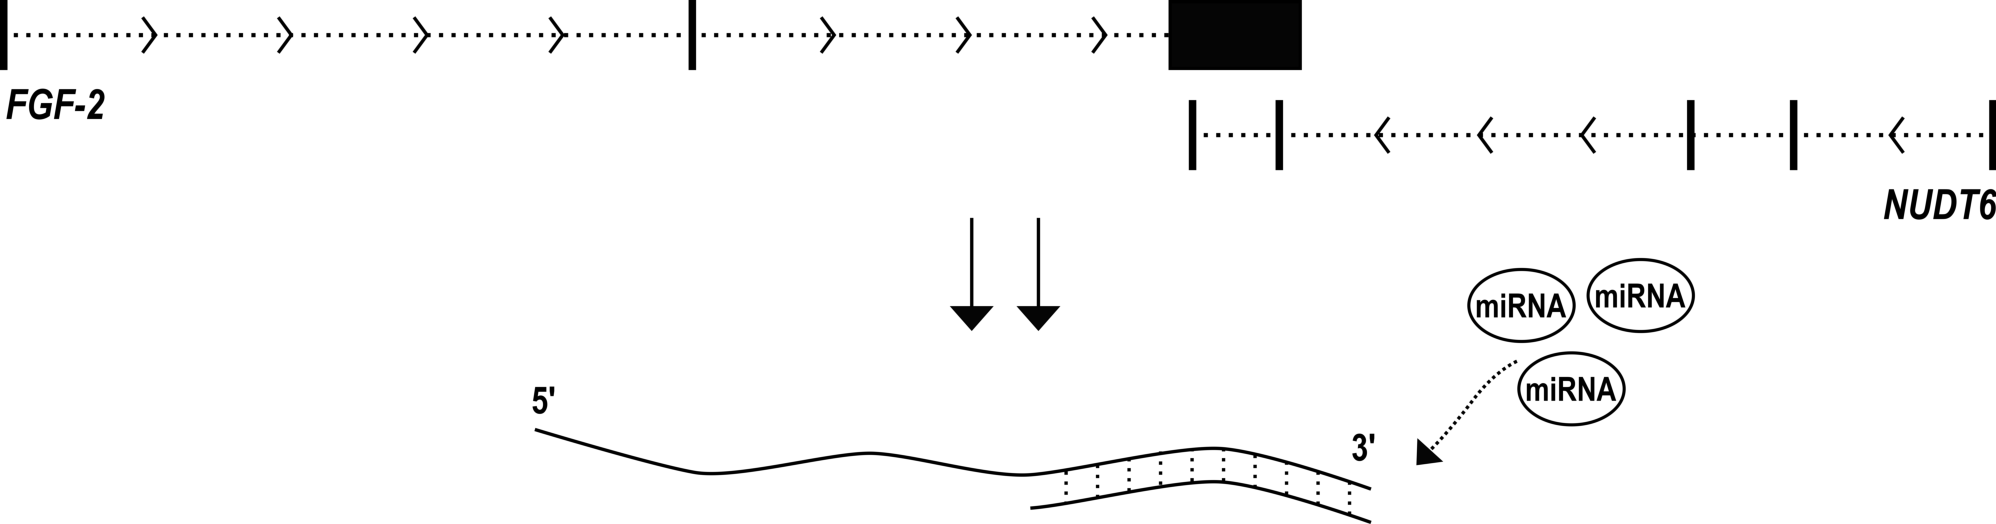
\includegraphics[scale=0.45]{figures/NUDT6.pdf}
\caption{The partial overlap of \emph{FGF-2} by the protein-coding gene \emph{NUDT6} regulates \emph{FGF-2} expression by forming double-stranded RNA duplexes reducing stability and translation efficiency. Arrows denote direction of transcription.}
\label{Figure 1-8: }
\end{figure}
%%%%%%%%%%%%%%%%%%%%%%%%%%%%%%%%%%%%%%%%%%%%%%%%%%%%%%

\subsection{\textit{Kcnq1ot1}}

\textit{Kcnq1ot1}, also known as \textit{Lit1}, is a 92 kbp lncRNA that emerges from intron 11 of \textit{Kcnq1} \cite{Lee1997,Smilinich1999}. The \textit{Kcnq1} imprinting cluster encompasses 10-12 imprinted maternally expressed protein-coding genes. \textbf{Figure \ref{Figure 1-9: }} shows that methylation of the maternal \textit{Kcnq1ot1} promoter restricts expression of the antisense lncRNA to the paternal allele \cite{Mancini-Dinardo2006}. Currently, there are two hypotheses for the imprinting mechanism of the \textit{Kcnq1} imprinting cluster: (1) direct silencing by \textit{Kcnq1ot1} recruits and propagates repressive factors \cite{Thakur2004}, (2) the regulatory elements produced by the transcription of \textit{Kcnq1ot1} recruits and propagates chromatin repressive factors \cite{Golding2011,Shin2008}. While there is evidence to support both hypotheses, recent work by Schultz and company suggest that it is the regulatory elements generated from the transcription of \textit{Kcnq1ot1} that are responsible for silencing the \textit{Kcnq1} imprinting cluster \cite{Schultz2015}.

By integrating publicly available sequencing data for the \textit{Kcnq1ot1} region, Schultz and company observed extensive processing of \textit{Kcnq1ot1} resulting in enhancer- and promoter-associating RNAs. These sequences line up to the poly(A)-sequencing sites observed in the mm9 UCSC genome assembly \cite{Kent2002} generated at Merck Research Laboratories. Additionally, Schultz and company confirmed multiple independent RNAs transcribed from the \textit{Kcnq1ot1} region using a combination of 5’ rapid amplification of cDNA ends (RACE) and chromosome conformation capture (3C) assay, and demonstrated that at least one of these RNAs directly interacted with the \textit{Kcnq1} promoter in the heart. Furthermore, when this transcription-rich region was deleted, imprinting was lost in the \textit{Kcnq1} imprinting cluster, altogether suggesting the region acts as a long-distance silencer.

%%%%%%%%%%%%%%%%%%%%%%%%%%%%%%%%%%%%%%%%%%%%%%%%%%%%%%
\begin{figure}[!ht]
\centering
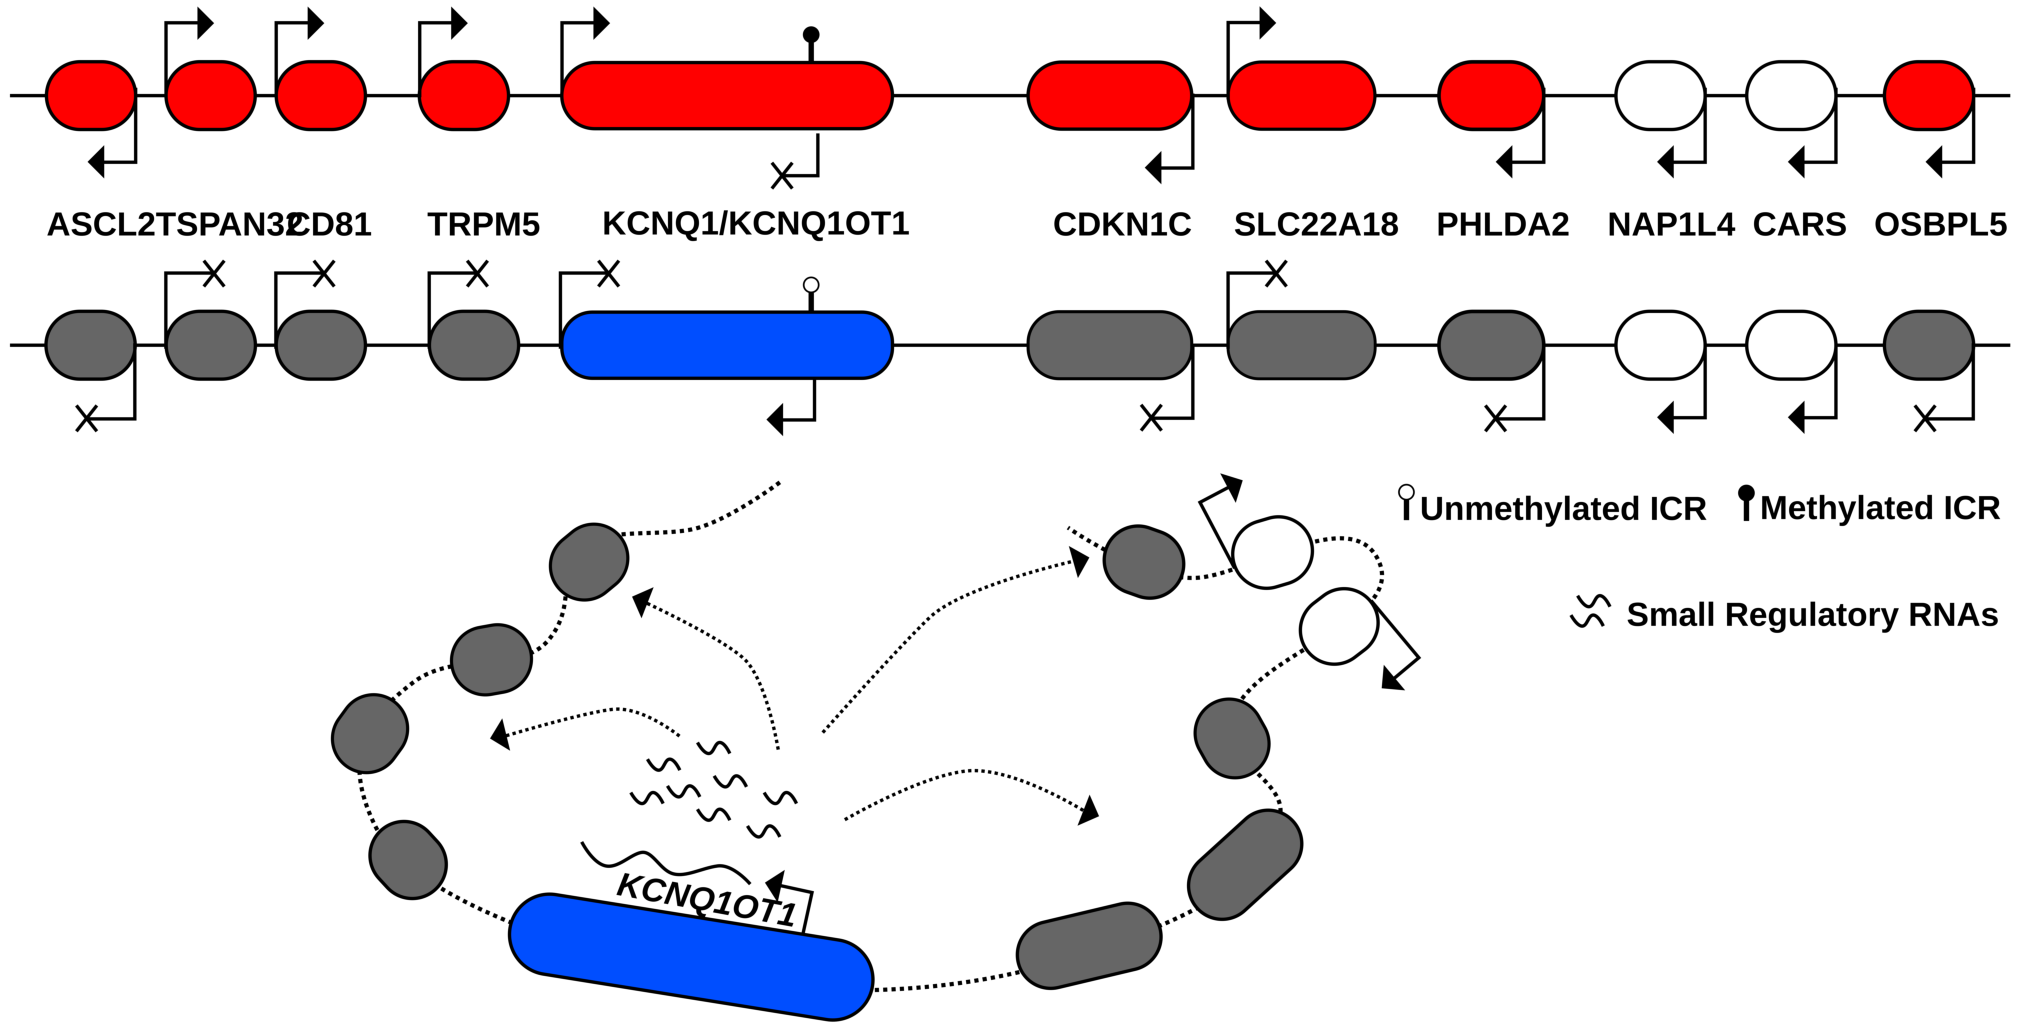
\includegraphics[scale=0.44]{figures/KCNQ1OT1.pdf}
\caption{Long range silencing of the \emph{KCNQ1} imprinting gene cluster is due to \emph{KCNQ1OT1}. It is proposed that processing of \emph{KCNQ1OT1} results in small regulatory RNAs, which interact with the imprinted genes causing silencing. Maternal allele (red), paternal allele (blue), silenced genes (gray), and non-imprinted genes (white). Arrows denote the direction of transcription.}
\label{Figure 1-9: }
\end{figure}
%%%%%%%%%%%%%%%%%%%%%%%%%%%%%%%%%%%%%%%%%%%%%%%%%%%%%%

\subsection{\textit{BACE1-AS}}

The antisense transcript of \textit{BACE1} (\textit{BACE1-AS}), a $\sim$2 kbp lncRNA, is transcribed from the \textit{BACE1} gene (beta-site amyloid precursor protein (APP)-cleaving enzyme 1), which is central to the pathogenesis of Alzheimer's disease. The lncRNA is a fully processed transcript that is highly expressed in Alzheimer's disease brains with two polyadenylated splice variants observed in human and mouse \cite{Faghihi2008}. Additionally, \textit{BACE1-AS} prevents microRNA-induced translational repression by competing with miR-485-5p binding of \textit{BACE1} in a tightly regulated system for BACE1 protein \cite{Faghihi2010}. When \textit{BACE1-AS} binds to \textit{BACE1}, it forms double-stranded RNA (dsRNA) duplexes that increase the stability of \textit{BACE1} as shown in \textbf{Figure \ref{Figure 1-10: }}. As a result, elevated levels of \textit{BACE1-AS} increase \textit{BACE1} expression creating a post-translational feed forward loop.

%%%%%%%%%%%%%%%%%%%%%%%%%%%%%%%%%%%%%%%%%%%%%%%%%%%%%%
\begin{figure}%[!ht]
\centering
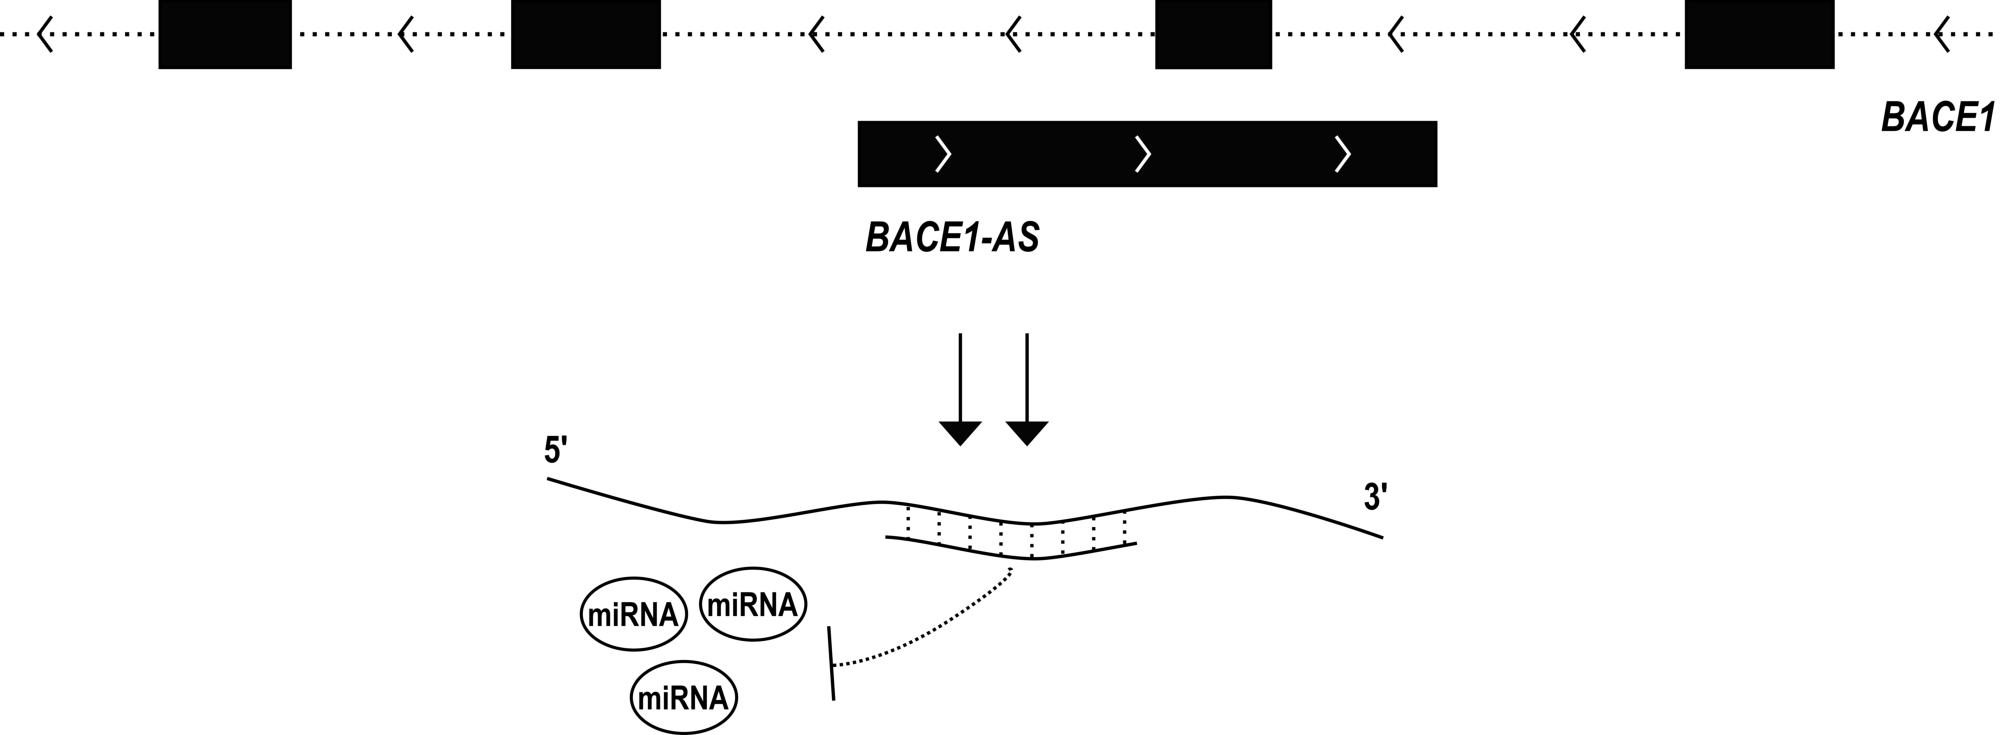
\includegraphics[scale=0.45]{figures/BACE1-AS.pdf}
\caption{\emph{BACE1-AS} increases stability of \emph{BACE1} via dsRNA duplexes. This increase in \emph{BACE1} stability results in increased protein levels of BACE1 creating a post-translational feed forward loop. Arrows denote the direction of transcription.}
\label{Figure 1-10: }
\end{figure}
%%%%%%%%%%%%%%%%%%%%%%%%%%%%%%%%%%%%%%%%%%%%%%%%%%%%%%

\subsection{\textit{BDNF-AS}}

The antisense transcript to brain-derived neurotrophic factor (\textit{BDNF-AS}) is a 191 kbp transcript with twelve splicing variants \cite{Pruunsild2007}. The first four exons of \textit{BDNF-AS} are downstream \textit{BDNF}, while the remaining exons overlap coding and introns of \textit{BDNF} \cite{Pruunsild2007}. The \textit{BDNF} gene, which plays an important role in peripheral neurons, neuron size, and arborisation, is a complex gene with 11 exons and 9 unique promoters resulting in 17 spliced transcripts with different 5' and 3' UTRs \cite{Modarresi2012,Pruunsild2007}. The partially conserved antisense transcript forms dsRNA duplexes with \textit{BDNF} mRNA in the brain resulting in the recruitment of EZH2 (enhancer of zeste homolog 2) and PRC2 to the promoter of \textit{BDNF} \cite{Modarresi2012} as depicted in \textbf{Figure \ref{Figure 1-11: }}. Thus, knockdown of the antisense results in increased mRNA and protein levels of BDNF.

%%%%%%%%%%%%%%%%%%%%%%%%%%%%%%%%%%%%%%%%%%%%%%%%%%%%%%
\begin{figure}[!ht]
\centering
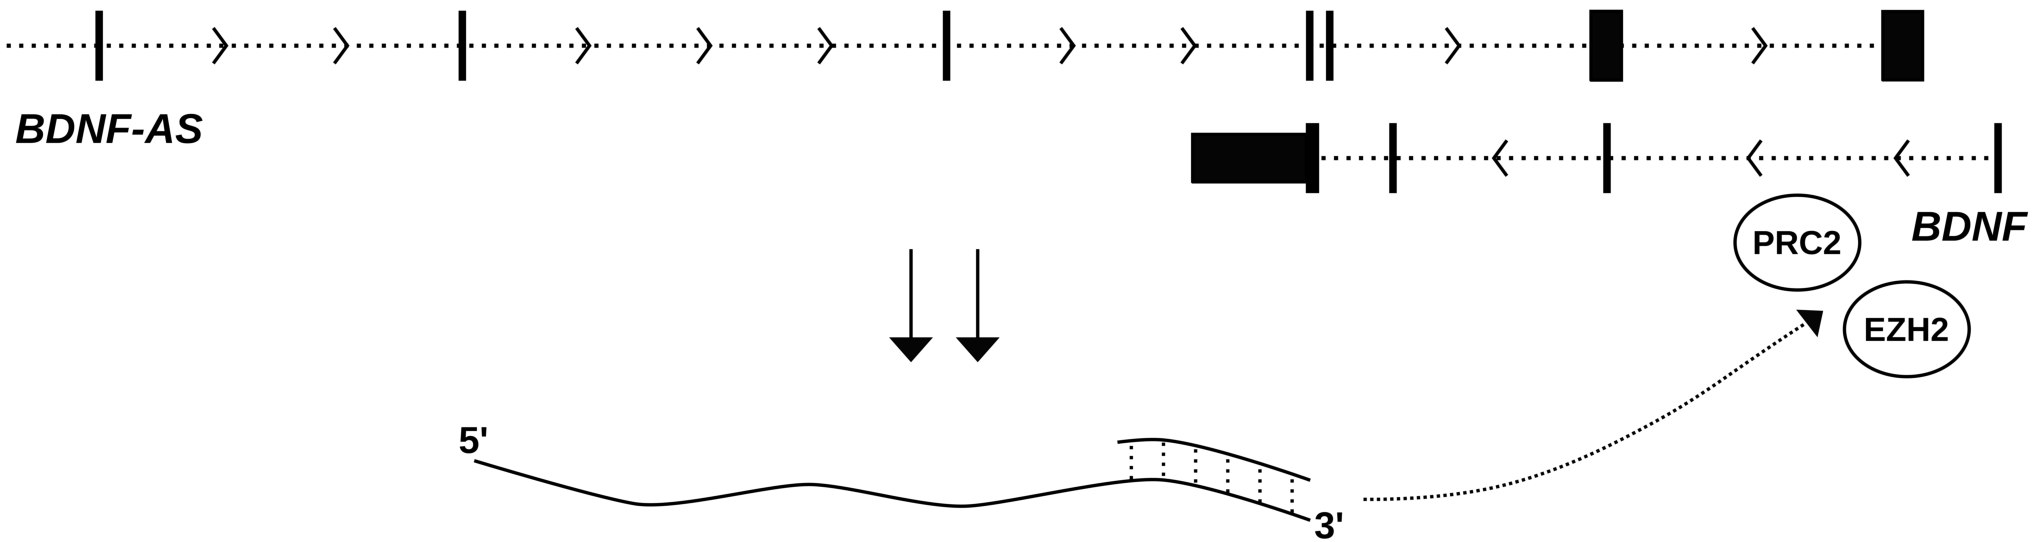
\includegraphics[scale=0.44]{figures/BDNF.pdf}
\caption{\emph{BDNF-AS} regulates \emph{BDNF} gene expression by forming double-stranded RNA resulting in the recruitment of chromatin modeling factors to the promoter of \emph{BDNF}. Arrow denotes the direction of transcription.}
\label{Figure 1-11: }
\end{figure}
%%%%%%%%%%%%%%%%%%%%%%%%%%%%%%%%%%%%%%%%%%%%%%%%%%%%%%

\subsection{\textit{Ube3a-AS}}

The \textit{Ube3a} antisense transcript is a part of a paternally expressed large transcriptional unit ($>$ 1000 bp) that initiates upstream of the PWS-IC from the \textit{Snurf/Snrpn} promoter \cite{Landers2004,Runte2004}. An unusual result of \textit{Ube3a-AS} being a part of this large transcriptional unit is its lack of a unique promoter. As such, its regulatory control for neuronal specific expression remains unclear. Moreover, how or why \textit{Ube3a-AS} regulates \textit{Ube3a} is still a mystery as very little is known about \textit{Ube3a-AS}, besides the fact that it is sufficient to imprint \textit{Ube3a} \cite{Chamberlain2001,Meng2012,Powell2013}.

There is no methylation at the promoter of \textit{Ube3a} or anywhere else within paternal \textit{Ube3a} \cite{Chamberlain2001,Dindot2009,Kishino2006}. In fact, paternal \textit{Ube3a} has been shown to be expressed; its transcription terminates between exon 4 and 5 \cite{Meng2013,Numata2011}. Although paternal \textit{Ube3a} is not currently known to produce a transcript, this partial expression is in stark contrast to the other well-studied antisense lncRNAs. One explanation of \textit{Ube3a} sense/antisense expression is that the transcriptional machinery for both transcripts collide causing transcription to terminate between exon 4 and 5 \cite{Meng2013}. In this model depicted in \textbf{Figure \ref{Figure 1-12: }A}, \textit{Ube3a-AS} transcription would generate high levels of torsional stress leading to stalling of transcriptional elongation complexes and silencing of \textit{Ube3a}.

With this model, it would be expected that transcription would stall at different places throughout \textit{Ube3a}; however, this is not the case. In two independent studies, biallelic expression of \textit{Ube3a} ends at one specific location \cite{Meng2013,Numata2011}. Additionally, Numata and company demonstrated \textit{Ube3a-AS} expression upstream \textit{Ube3a} using their SNP analysis, which indicates that \textit{Ube3a-AS} continues transcription beyond the suggested collision point. The termination of \textit{Ube3a-AS} upstream \textit{Ube3a} aligns with polyadenylation sites from Merck Research Laboratories’ poly(A)-sequencing data observed in mm9 UCSC Genome Browser \cite{Kent2002}. Moreover, the transcriptional termination of biallelic expression of \textit{Ube3a} also aligns with Merck poly(A)-sequencing data. Altogether, these observations suggest an alternative mechanism of silencing, where the transcription of \textit{Ube3a-AS} leads to alternative polyadenylation within the intron between exon 4 and 5 of \textit{Ube3a} that terminates transcription shown in \textbf{Figure \ref{Figure 1-12: }B}.

%%%%%%%%%%%%%%%%%%%%%%%%%%%%%%%%%%%%%%%%%%%%%%%%%%%%%%
\begin{figure}[!ht]
\centering
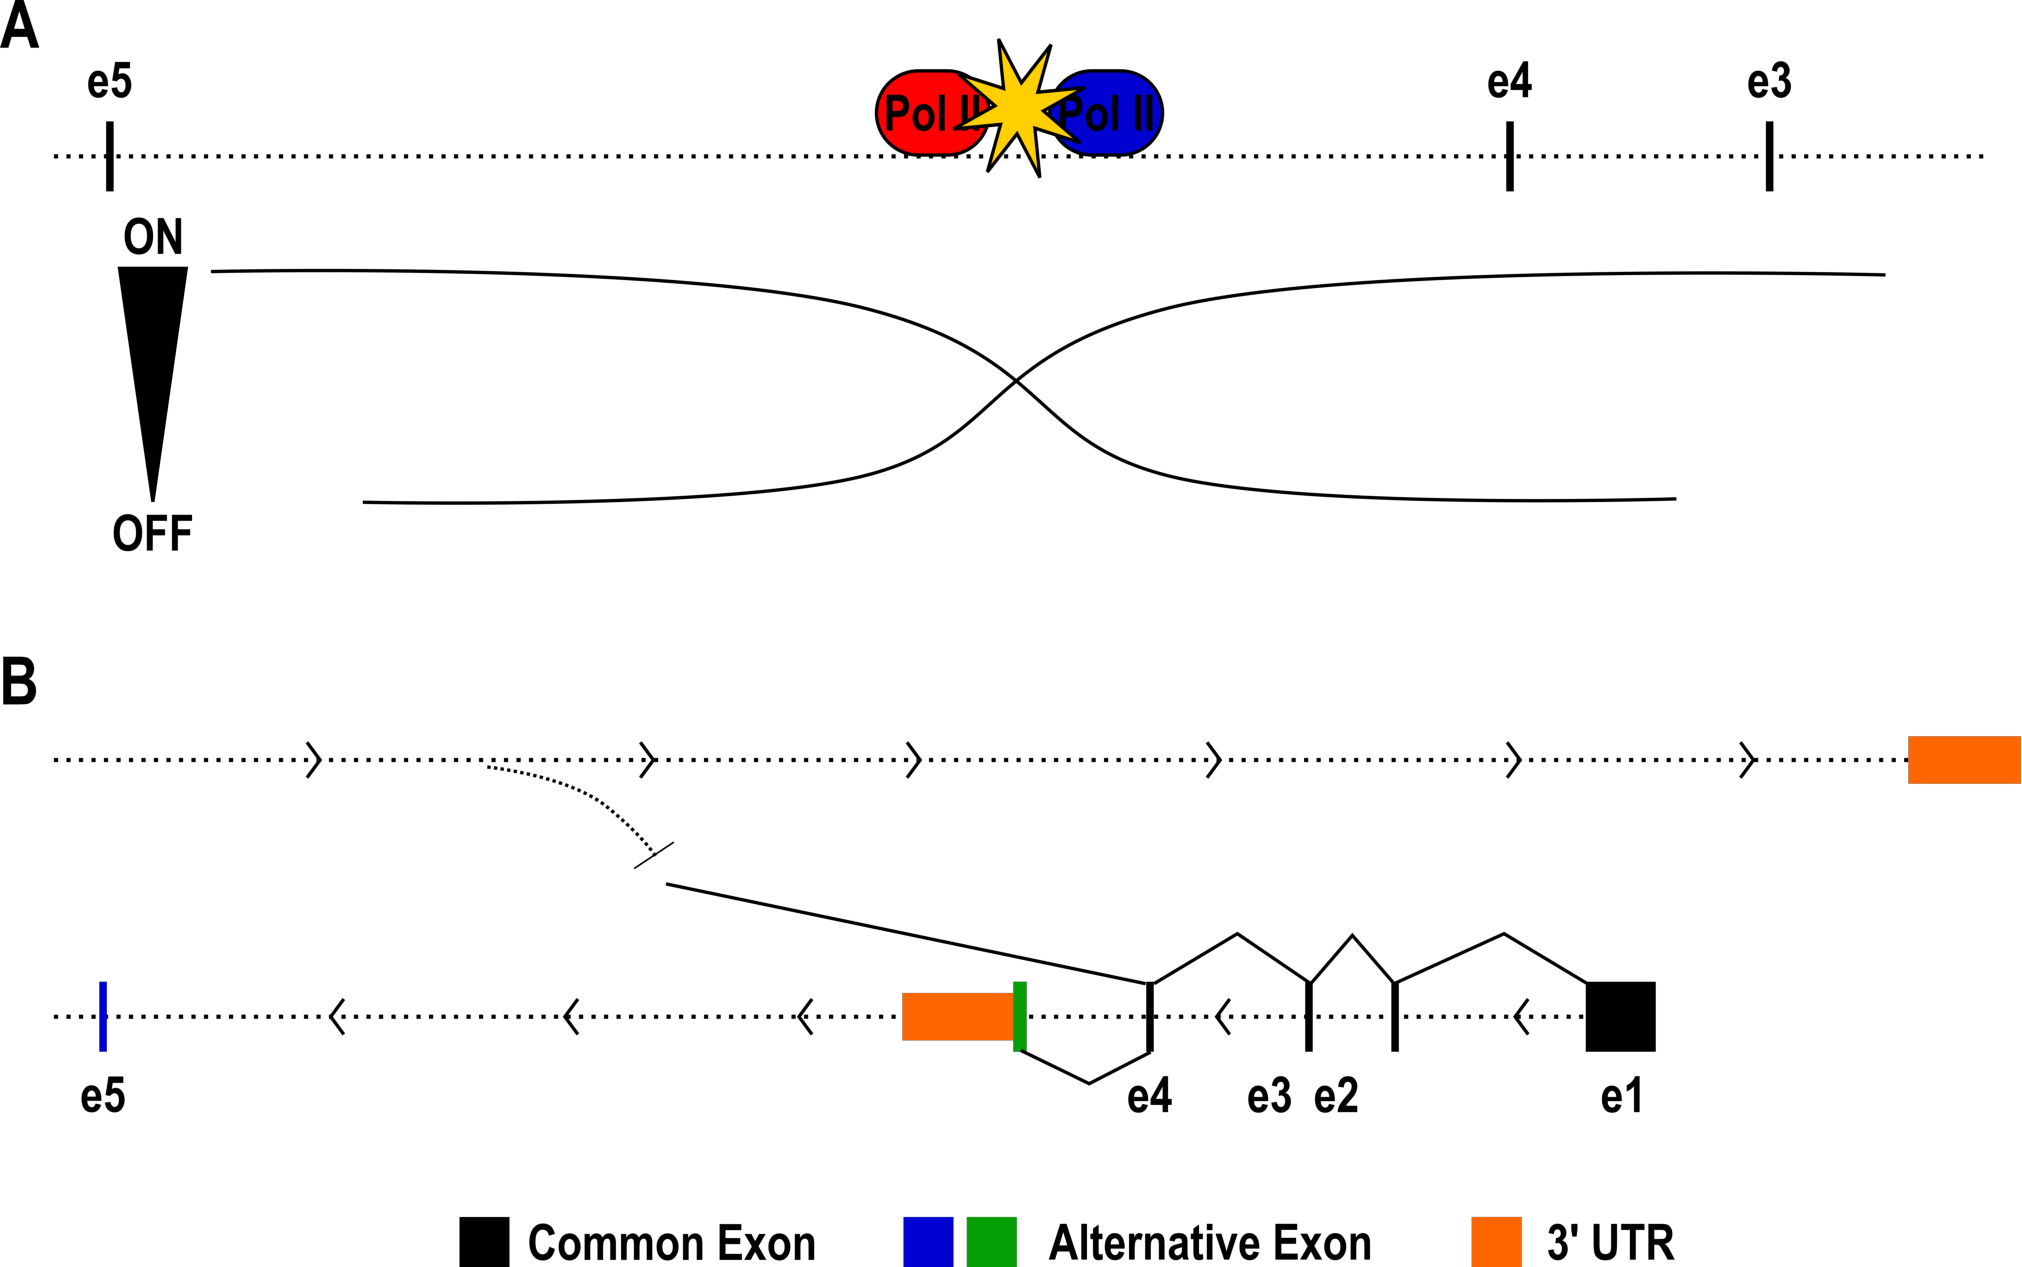
\includegraphics[scale=0.45]{figures/Ube3a-AS_mechanism.pdf}
\caption{\emph{UBE3A-AS} regulates paternal \emph{UBE3A} expression in neurons. \textbf{A)} Transcriptional collision model for \emph{UBE3A-AS} regulation of \emph{UBE3A}. \textbf{B)} Purposed alternative splicing model for \emph{UBE3A-AS} regulation of \emph{UBE3A}. Polymerase II (Pol II), antisense Pol II in red and sense Pol II in blue. Arrows denote the direction of transcription.}
\label{Figure 1-12: }
\end{figure}
%%%%%%%%%%%%%%%%%%%%%%%%%%%%%%%%%%%%%%%%%%%%%%%%%%%%%%

\section{Concluding Remarks}

This paper has reviewed the importance of \textit{UBE3A} and suggested a possible function for its antisense transcript outside of imprinting of \textit{UBE3A} as a reason for its imprinting. Recent studies in our laboratory have demonstrated that \textit{Ube3a} is not imprinted to regulate its gene expression in neurons \cite{Hillman2017}. Moreover, the imprinting of \textit{Ube3a} has no overall effect on \textit{Ube3a} expression suggesting that the importance of imprinting \textit{Ube3a} may lie in its antisense transcript, \textit{Ube3a-AS} \cite{Hillman2017}. Long non-coding RNAs, like \textit{Ube3a-AS}, are diverse in structure and function. It is possible that \textit{Ube3a-AS} also functions in a complex manner. It is clear from this review that more investigation is needed to elucidate \textit{Ube3a-AS} function and its connection to \textit{Ube3a} imprinting.

The implications of \textit{UBE3A-AS} having a function impacts therapeutic intervention for the diseases of the area, Angelman syndrome, Prader-Willi syndrome and Chromosome15q duplication syndrome. Specifically, for AS where the only current treatment options target the reactivation of paternal \textit{UBE3A} via disruption of \textit{UBE3A-AS} \cite{Bailus2016,Elgersma2007,Huang2012,Meng2013,Meng2015,Shi2015,Silva-Santos2015}, any possible function of the antisense transcript will need to be extensively considered. As such, a better understanding of imprinting of \textit{UBE3A} may help facilitate drug development for Angelman syndrome, while possibly mitigating the ramifications for transcriptional silencing of \textit{UBE3A-AS}.

%%  LocalWords:  UBE3A antisense lncRNA genomic ubiquitin ligase PWS
%%  LocalWords:  epigenetic Dup15q OMIM RNAs snoRNAs HBII E3A E3 E1
%%  LocalWords:  E2 HECT SNURF SNRPN SNORD115 IPW ICR cis ICRs DMR IC
%%  LocalWords:  CpG ATP10A Hillman et al upregulated SNRPB
